\chapter{Advanced strategies for Privacy-Enhancing Machine Learning}

This final chapter delves into advanced strategies for enhancing privacy in machine learning, spotlighting two pivotal concepts: Differential Privacy and Generative Models. Each of these strategies offers unique mechanisms for ensuring that sensitive data remains secure and confidential throughout the machine learning lifecycle.

\textbf{Differential Privacy} provides a robust mathematical framework for ensuring that the output of a machine learning model does not compromise the privacy of individual data points. By incorporating controlled noise into the data or the learning process, differential privacy aims to make it difficult for adversaries to infer any specific information about an individual, even if they have access to the model's output.

\textbf{Generative Models}, like Variational Autoencoders (VAEs) and Generative Adversarial Networks (GANs), offer innovative approaches to creating synthetic data that can be used for training machine learning models. These synthetic datasets can mimic the statistical properties of real data without exposing any sensitive information, providing a valuable tool for data sharing and collaborative research without compromising privacy.

This chapter will provide a comprehensive overview of these advanced privacy-enhancing strategies, discussing their principles, implementations, and the challenges associated with their deployment. By integrating these techniques, we can build more secure and privacy-preserving machine learning systems that respect and protect user data in an increasingly data-driven world.

\section{Differential Privacy}


Differential Privacy (DP) is a formal framework designed to ensure the privacy of individuals in a dataset. It operates on the principle of introducing randomness to the data or the analysis process to mask the presence or absence of any single individual. This makes it difficult for adversaries to glean specific information about any individual, even if they have extensive background knowledge. Differential Privacy has become a cornerstone of privacy-preserving data analysis, used by major organizations like Google, Apple, and the US Census Bureau.

\subsection{Principles of Differential Privacy}

The core idea of Differential Privacy is to provide guarantees that the output of a function (algorithm) will be roughly the same whether or not any single individual's data is included in the input dataset. This is typically achieved by adding carefully calibrated noise to the data or to the function's output. The degree of noise is governed by two parameters: $\epsilon$ (epsilon) and $\delta$ (delta).

\begin{itemize}
    \item \textbf{$\epsilon$ (Epsilon):} Represents the privacy loss parameter. Smaller values of $\epsilon$ indicate stronger privacy guarantees, but potentially less accurate results.
    \item \textbf{$\delta$ (Delta):} Represents the probability that the privacy guarantee does not hold. A smaller $\delta$ value indicates a higher level of confidence in the privacy guarantee.
\end{itemize}

Mathematically, a randomized algorithm $A$ is $(\epsilon, \delta)$-differentially private\footnote{Sometimes, when $\delta=0$ is referred as \textit{pure differentially private}, and otherwise as \textit{approximate differentially private} } if for any two datasets $D$ and $D'$ that differ by only one element, and for any possible output $S$ of the algorithm:

\[ Pr[A(D) = S] \leq e^\epsilon \times Pr[A(D') = S] + \delta \]

This definition ensures that the inclusion or exclusion of a single individual’s data does not significantly affect the outcome, thereby preserving privacy. Therefore, this mathematical framework guarantees that anyone seeing the result of a differentially private analysis will make the same inference about any individual's private information, whether that individual's information in included or not. \cite{wood2018}
Note that $\epsilon=\delta=0$ is equivalent to absolute privacy: the algorithm $A$ is independent of the data. Therefore, there is no accuracy in the queries and this algorithm would be useless for a data analysis.


\subsection{Private Aggregation of Teacher Ensembles}
In \cite{fredrikson2015}, it is shown that a model inversion attack that exploits confidence values revealed along with prediction would lead to an unexpected privacy issues. In order to avoid this there are several techniques, we will focus on one algorithm based in differential privacy that provides strong privacy guarantees for training data.
For this section, it will be explained the algorithm Private Aggregation of Teacher Ensembles (PATE) \cite{papernot2017}, which trains multiple models (teachers) on disjoint datasets (local data from parties, as explained in Section \ref{ch:Federated_Learning}). These models remain local (like in a federated learning setting) and act as teachers for a \textit{student} model.

\begin{figure}[H]
    \centering
    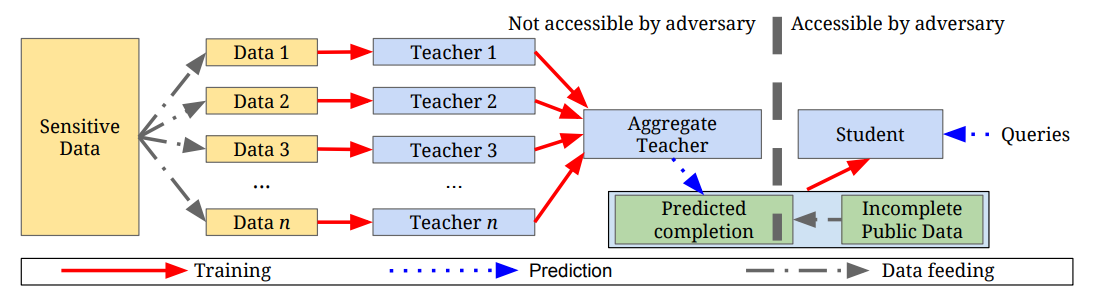
\includegraphics[scale=.35]{figures/4-Advanced_Strategies/PATE_scheme.png}
    \caption{Overview of PATE: an ensemble of teachers is trained on disjoint subsets of the sensitive data and a student model is trained on public data labeled using the ensemble. Source: \cite*{papernot2017}}
\end{figure}

Suppose we have a public dataset $\{\mathbf{x}, y\}$ where $\mathbf{x}$ denotes the features and $y$ the set of labels. We partition the data in $n$ disjoint sets following the IID hypothesis $D^i$, $i=1,...,n$ and each teacher model trains separately on each set, obtaining $n$ classifiers $f_i$. We then deploy them as an ensemble making predictions on unseen inputs $\mathbf{x}$ by aggregating into a single prediction the outputs $\{f_i(\mathbf{x})\}_{i=1}^n$.
The privacy guarantees of the teacher ensemble stems from the aggregation step: let $m$ be the number of classes in the classification task, the label count for a given class $j \in [m]$ and $n_j (\mathbf{x}) = |\{i \colon i \in [n], f_i(\mathbf{x}) = j\}|$ the number of teaches that assigned class $j$ to input $\mathbf{x}$. Under a majority vote where the label with the largest count is the final prediction, the ensemble's decision may depend on a single teacher's vote (if two labels have a vote count differing by at most one). A random noise is added to the vote count $n_j$: $f(x) = \arg \max_j \bigl\{ n_j (\mathbf{x} + Lap\Bigl( \frac{1}{\gamma} \Bigr)) \bigr\}$, where $\gamma$ is a privacy parameter (not exactly $\epsilon$, although \cite{papernot2017} explains its relationship in Theorem 2), and $Lap(\gamma)$ is the Laplacian distribution with location $0$ and scale $\gamma$. a larger $\gamma$ leads to a stronger privacy guarantee but in a degradation of the accuracy, since the maximum $f$ can differ from the true majority. From the Fundamental Law of Information Recovery \cite{dwork2013}, the noise required would increase as we make more predictions, besides the teachers have been trained on raw data, being susceptible of a membership inference attack \cite{shokri2017}.
For this reason, another model (the student) is trained using a fixed number of labels predicted by the teacher ensemble. The student model is trained on unlabeled data, some of which it's labeled using the aggregation mechanism. Unlabeled inputs are used in unsupervised learning to estimate a good prior for the distribution while the labeled inputs are then used for supervised learning.  Over time, the student learns to generalize from these noisy, aggregated answers, resulting in a model that performs well while preserving the privacy of the original training data.\\

This algorithm has some limitations: it's computationally expensive since it needs to train multiple teacher models, each on a different subset of data. In the aggregation step, it needs to get the response from the teachers, therefore is not suitable for real-time applications.
Moreover, the number of teacher models and the privacy constants add more hyperparameters to the ML workflow, requiring more tuning to balance the model performance and the privacy. It also needs to distribute the data between the teachers in a IID setting, which means we need to have access to some kind of public data (which may not be the case in most real scenarios).\\
Although it was one of the first and most known algorithm in the PEML community, there are other algorithms and approaches more suitable for a broader use cases. However, because of its simplicity it's still used, and some variants have been proposed: \cite{long}, \cite{jordon2019}.

\subsection{Differentially Private SGD}
Recall from Section \ref{sec:optimizer} that for complex NN $J(\theta; x)$ is usually non-convex and difficult to minimize, and in practice a mini-batch stochastic gradient descent (SGD) or some variant is used. In this algorithm, a batch $B$  of random samples is used to compute $\mathbf{g} = \frac{1}{|B|} \sum_{(x,y) \in B} \nabla_\theta J(\theta; x)$, and estimation to the gradient $\nabla_\theta J(\theta)$.\\
In order to protect the privacy of the training data, it can be modified the SGD algorithm: after computing $\nabla_\theta J(\theta, x)$ for a batch $B$, we clip the $l_2$ norm of each gradient, compute the average, add noise and update the weights in a direction slightly modified by the noise. This approach can be studied in detail in \cite{abadi2016}, where the computation of the overall privacy cost $(\epsilon, \delta)$ is explained.


\begin{algorithm}[H]
  \caption{DP-SGD}
  \label{alg:DP_SGD}
  \begin{algorithmic}[1]
    \Require{Data $\{(x_i,y_i)\}_{i=1}^N$, a loss function $J(\theta)$, a learning rate $\eta_t$, a noise scale $\sigma$ and a gradient norm bound $C$}
    \State Initialize $\theta$ randomly.
    \For {each step $t$}
      \State Take a batch $B \subset \mathcal{B}$ of samples
      \State For sample $i$ in $B$, compute $g_t(x_i) = \nabla_{\theta_t} J(\theta_t, x_i)$
      \State Clip gradient: $g_t(x_i) = g_t(x_i)/\max \bigl( 1, \frac{||g_t(x_i)||_2}{C} \bigr)$
      \State Add noise: $g_t = \frac{1}{|B|} \bigl( \sum_i g_t(x_i) + N(0, \sigma^2 C^2 \boldsymbol{I}) \bigr)$
      \State $\theta_{t+1} = \theta_t - \eta_t g_t$
    \EndFor
  \end{algorithmic}
\end{algorithm}

A direct implementation of Algorithm \ref{alg:DP_SGD} would be impractical in frameworks like PyTorch or Tensorflow, since they don't expose intermediate computations, including per-sample gradients (only give access to the gradients averaged over a batch). Instead of bypass this limitation with batch sizes of 1 (which would be quite inefficient), we recommend the framework Opacus\footnote{\url{https://github.com/pytorch/opacus}} explained in \cite{yousefpour2022}, which makes the implementation of this algorithm (and other DP related algorithms) trivial to implement\footnote{For example, the implementation of Algorithm \ref{alg:DP-SGD} using a MLP on MNIST dataset can be seen in \url{https://github.com/pytorch/opacus/blob/main/examples/mnist.py}}.

\subsection{Applications of Differential Privacy}

Differential Privacy has a wide range of applications, particularly in scenarios where sensitive data is analyzed. Some notable examples include:

\begin{itemize}
    \item \textbf{Statistical Databases:} Differential Privacy can be used to release summary statistics from sensitive databases without compromising individual privacy.
    \item \textbf{Machine Learning:} Differential Privacy techniques can be applied to train machine learning models on sensitive data, ensuring that the models do not reveal information about individual training examples.
    \item \textbf{Census Data:} The US Census Bureau has adopted Differential Privacy to protect the privacy of respondents while releasing demographic statistics \cite{bureau}.
\end{itemize}

By incorporating Differential Privacy, organizations can provide robust privacy guarantees while still gaining valuable insights from their data. The balance between privacy and utility is crucial, and Differential Privacy offers a principled approach to achieving this balance.

\subsection{Challenges and Considerations}

While Differential Privacy offers strong privacy guarantees, it also presents several challenges:

\begin{itemize}
    \item \textbf{Parameter Selection:} Choosing appropriate values for $\epsilon$ and $\delta$ is critical and often context-dependent. Lower values provide better privacy but can significantly impact data utility.
    \item \textbf{Sensitivity Calculation:} Accurately determining the sensitivity of a query is essential for effective implementation. Overestimating sensitivity can lead to excessive noise, while underestimating it can compromise privacy.
    \item \textbf{Complex Queries:} Implementing Differential Privacy for complex queries, such as those involving joins or non-linear transformations, can be challenging. The Fundamental Law of Information Recovery states that overly accurate answers to too many questions will destroy privacy (see Section 8.1 of \cite{dwork2013} for a formal proof)
\end{itemize}

Despite these challenges, Differential Privacy remains a powerful tool for privacy-preserving data analysis. Ongoing research and development continue to enhance its practicality and effectiveness, making it a cornerstone of modern privacy-preserving technologies.




\section{Generative Models}

In Privacy Enhancing Machine Learning, generative models are being used to capture joint distributions of data in order to obtain synthetic samples without using real data. This can be used effectively to initialize deep learning models, perform data analysis, or apply it in competitions where models are initially validated using synthetic data and later tested (privately) with the original data.\\
The approach of this section will be to test the feasibility of using generative adversarial networks to extract data features and approximate their distribution. This is not done to train discriminative models with synthetic data, but rather to use synthetic data for tuning and designing models, thus enabling remote training (the model is trained locally where the data reside) without needing access to the original data, following the philosophy of Federated Learning (see section \ref{ch:Federated_Learning}). Comparing and evaluating the design of a Federated Learning model is beyond the scope of this work; instead, the distributions of the original datasets and synthetic datasets will be compared and evaluated.\\
In summary, two datasets will be used to test the feasibility of using generated data to facilitate model training in a Federated Learning environment, without necessarily using this data in the final model training. The aim is to approximate the distribution of the original dataset (a very challenging task). This could be done in conjunction with other techniques such as data anonymization, but this work will focus solely on generative models, particularly GANs. To assess the quality of synthetic data, scatter plots, histograms, and metrics measuring similarity in marginal distributions will be used.\\
The GAN (Generative Adversarial Network) architecture was originally proposed in \cite{goodfellow2014}. Since then, there have been numerous variations and improvements, primarily focused on image generation. Although other generative models exist, such as diffusion models, the GAN architecture remains employed and studied. In its original definition, the architecture consists of two models: a generative model $G$ that approximates the data distribution, and a discriminator model $D$ that estimates the probability that a sample is real or synthetic (generated by $G$). Both $G$ and $D$ are MLP (Multi-Layer Perceptron) architectures; in the case of $G$, the output dimension must match that of the real data. The main idea is that during training, these two models compete: $G$ seeks to learn to generate realistic data that can deceive $D$, while $D$ aims to correctly distinguish between real and generated samples from $G$. The input vector for $G$ consists of random noise, for example, $z \sim N(\mathbf{0}, \sigma \mathbf{I})$; denoted as $G = G(z) = G(z; \theta_g)$, where $\theta_g$ represents the network weights. The discriminator takes as input a real or synthetic data vector $x$, denoted interchangeably as $D = D(x) = D(x; \theta_d)$. The (simplified) training process is as follows:\\
First, the weights of $G$ and $D$ are initialized randomly. During each epoch, real data ${x_1,...,x_m}$ and random noise ${z_1,...,z_m}$ are sampled, where $x_i$ and $z_i$ have the same dimensions, for example, $x_i, z_i \in \mathbb{R}^p, \quad p \in \mathbb{N}$. In the case of tabular data, it can occur, for instance, $x_i, z_i \in \mathbb{R}^p \times \mathbb{Z}^k, \quad p,k \in \mathbb{N}$, if the table consists of $p$ columns of real data and $k$ columns of integer data. It can also occur that the data are categorical: if the i-th column is categorical, the i-th component of the vector $x$ and $z$ will take values in a finite set $\Omega$ that can be numerically encoded. This will affect the exact definition of the initial (a priori) distribution of $z$.

Next, the batch of synthetic samples ${G(z_1),...,G(z_m)}$ is computed. Now $D$ receives both the batch of real data ${x_1,...,x_m}$ and the batch of synthetic data ${G(z_1),...,G(z_m)}$ and must distinguish between them. Therefore, $D$ is a discriminative (supervised) binary classification model; it classifies as 1 the data it confidently predicts as real and as 0 the synthetic data ($D$ outputs a probability between 0 and 1). Based on this classification, the discriminator's loss function is calculated, and $D$'s weights are adjusted to \textbf{minimize} this loss.

Next, another batch of synthetic data ${G'(z_1),...,G'(z_m)}$ is generated, and $G$'s loss is computed as it tries to deceive the discriminator (which has already been updated). $G$'s weights are updated to \textbf{maximize} this loss. This process is repeated iteratively until a stopping criterion is met, such as a maximum number of epochs.

Therefore, this involves the following min-max game:
\begin{equation}
\min_G \hspace{0.3 em} \max_D V(G,D) = E_{x \sim \rho_{\text{data}}(x)}[\log D(x)] + E_{z \sim \rho_z(z)}[\log(1 - D(G(z)))]
\label{eq:funcion_objetivo_GAN}
\end{equation}

The intuitive idea behind this formula is as follows: the ultimate goal of the architecture is for $\rho_z$ to converge to $\rho_{\text{data}}$, meaning that $G$ should approximate the theoretical data distribution perfectly (although $\rho_{\text{data}}$ is unknown and we only have a finite sample of data). To achieve this, we use $D$: if there were a perfect discriminator that could distinguish between real and synthetic data, we could use it to update the weights of $G$ and improve the generative model. The approach is to train both models simultaneously with the aim of achieving perfect models: where $D$ correctly classifies the data, maximizing the probability of classifying samples drawn from $\rho_{\text{data}}$ as real, and minimizing the probability of classifying samples generated by $G$ as real. This is expressed as:
\begin{equation*}
\max_D V(G,D) = E_{x \sim \rho_{\text{data}}(x)}[\log D(x)] + E_{z \sim \rho_z(z)}[\log(1 - D(G(z)))]
\end{equation*}

At the same time, given a discriminator $D$, we want $G$ to maximize the probability that $D$ classifies samples drawn from $\rho_z$ as real. This can be formulated as:
\begin{equation*}
\max_G V(G,D) = E_{z \sim \rho_z}[\log D(G(z))] \Leftrightarrow \min_G V(G,D) = E_{z \sim \rho_z} [\log(1 - D(G(z)))]
\end{equation*}

These two formulations lead us to (\ref{eq:funcion_objetivo_GAN}).\\
\textbf{Note:} In implementations, care is taken to ensure that the probability returned by $D$ is not exactly 0 or 1 to avoid $\log$ from approaching 0.\\

Taking this into account, we can now understand the expressions given in the original paper \cite{goodfellow2014} for updating the model weights. Let's start with $D$, which receives batches of real data ${x_1,...,x_m}$ and synthetic data ${G(z_1),...,G(z_m)}$. Stochastic gradient ascent is applied as follows:

\begin{equation*}
\theta_{d}' = \theta_d + \eta \frac{\partial }{\partial \theta_d} \left[ \frac{1}{m} \sum_{i=1}^m \left( \log D(x_i) + \log (1 - D(G(z_i))) \right) \right]
\end{equation*}

\textbf{Note:} We take the mean of individual losses, which represents the empirical risk: an estimation of the theoretical risk since we do not know the theoretical data distribution. I emphasize the $+$ sign, as our goal is to maximize.

For $G$, the weights are updated using stochastic gradient descent as follows:

\begin{equation*}
\theta_{g}' = \theta_g - \eta \frac{\partial}{\partial \theta_g} \left[ \frac{1}{m} \sum_{i=1}^m \log(1 - D(G(z_i))) \right]
\end{equation*}

\textbf{Note:} This is a simplified version of stochastic gradient methods. The original paper mentions using a variant with momentum (see section \ref{sec:optimizer}). There are many variations with different hyperparameters and features. A deliberately simplified terminology has been maintained.

Since both $G$ and $D$ are MLPs, gradients can be efficiently computed using the backpropagation algorithm.

For tabular datasets, certain particularities must be addressed (\cite*{xu2019}). In particular, we will use a variant of the original GAN: the Conditional GAN. We will consider features (columns) of both continuous and discrete data. The generator model must differentiate between the two; in the final layer, a $softmax$ activation function will be used for the discrete case and $tanh$ for the continuous case.

\begin{align*}
tanh(x) &= \frac{e^x - e^{-x}}{e^x + e^{-x}} \quad x \in \mathbb{R} \\
softmax (\mathbf{x})_j &= \frac{e^{x_j}}{\sum{i=1}^n e^{x_i}} \quad j=1,...,n \quad \mathbf{x} \in \mathbb{R}^n
\end{align*}

In a conditional GAN, both the generator and the discriminator also receive additional information, which can be in the form of class labels, specific features, or any other relevant information for the problem at hand. This additional information is provided as a condition for the generation of synthetic samples and the evaluation of their authenticity.\\
Introducing conditional information into a GAN allows for more specific control over the generation process. For example, in the case of image generation conditioned on certain class labels, a conditional GAN can generate images of a specific type, such as "cats" or "dogs," according to the label provided as the condition.\\
In the context of CTGAN (Conditional Tabular Generative Adversarial Networks), this additional information can be any relevant feature or set of features present in the original data. For example, if working with a tabular dataset containing information about bank customers, the additional information could include the customer's gender, age, account type, credit history, etc.\\
During the training process of the CTGAN, both the generator and the discriminator receive this additional information as a condition for the generation and evaluation of synthetic data. This means that the generator learns to generate synthetic samples that are not only statistically similar to the original data but also conditioned on specific values of the provided features.\\
For example, if one wants to generate synthetic data of bank customers with a certain age range and gender, this information can be provided as a condition to the CTGAN during the generation process. As a result, the CTGAN will be able to generate synthetic samples that follow the distributions of the conditioned features, which can be useful in various applications, such as generating balanced training data, preserving privacy, or conducting sensitive testing. In summary, CTGAN applies the principles of conditional GANs to the specific context of tabular data synthesis.\\
When working with tabular data instead of images, several aspects must be considered, such as continuous variables not typically following a normal distribution; in fact, they may follow a multimodal distribution (having more than one peak of maximum density). Additionally, there can be issues of imbalanced features (for example, in the case of banking data, a binary variable determining default status is often very imbalanced, as most customers are not defaulters).\\
To numerically evaluate the synthetic datasets, the KSComplement and TVComplement metrics from the \textit{SDMetrics} library will be used. The KSComplement metric calculates the similarity (of the marginal distribution) between two columns, one real and one synthetic. It uses the Kolmogorov-Smirnov statistic, which measures the maximum difference between two cumulative probability distributions, yielding a value between 0 and 1. KSComplement returns $1-KS$, meaning the closer to 1, the more similar the distributions. This metric will be used for continuous variables. For categorical variables, the TVComplement metric from the same library will be used, which also measures the similarity between two marginal distributions. It calculates the frequentist probability of each class and sums the absolute differences for each class. The metric returns $1-\text{result}$, so the closer the value is to 1, the better the distributions match.\\

\textbf{Results:}

For the implementation, the CTGAN library in Python has been used. This library addresses the problem of non-Gaussian and multimodal data through variational Gaussian mixture models to estimate complex distributions. Explaining Gaussian mixtures is beyond the scope of this work, but \cite*{bishop2006} has been used as a reference for this type of model.\\
A total of 2 datasets have been used to check the performance of CTGAN. The first consists of a dataset generated by myself, composed of two columns $x$ and $y$ that follow a normal distribution $N(\mu, \Sigma)$, where $\mu = \begin{pmatrix}
0 \\
0
\end{pmatrix}$ and $\Sigma = \begin{pmatrix}
1 & 0.5 \\
0.5 & 1
\end{pmatrix}$, meaning they are positively correlated variables. The third column is a categorical feature with 5 classes encoded with numbers from 0 to 4. These classes have been generated using the probability vector $p=(0.3, 0.2, 0.4, 0.07, 0.03)$. A thousand samples of this dataset have been generated, and CTGAN was trained for 3000 epochs. This is a somewhat arbitrary stopping criterion after observing the objective function graphs, as the loss curves of $G$ and $D$ oscillate and do not reach Nash equilibrium. Theoretically, the optimum is reached when $D = 1/2$, that is, when it is unable to differentiate between real and synthetic data and determines this randomly. The goal of this work is not to train the best possible model but to study its feasibility according to the privacy objectives set.

A thousand rows of $\rho_z$ were sampled:


\begin{figure}[htbp]
    \centering
    \begin{minipage}[b]{0.4\textwidth}
      \centering
      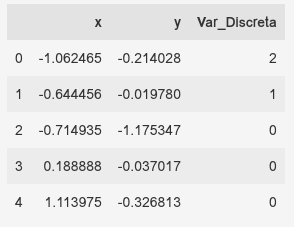
\includegraphics[width=0.6\textwidth]{figures/4-Advanced_Strategies/Ejemplo_Dataset_1_Real.png}
      \caption{Real samples}
    \end{minipage}
    \hfill
    \begin{minipage}[b]{0.4\textwidth}
      \centering
      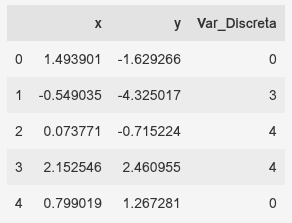
\includegraphics[width=0.6\textwidth]{figures/4-Advanced_Strategies/Ejemplo_Dataset_1_Sintetico.png}
      \caption{Synthetic samples}
    \end{minipage}
\end{figure}

\begin{figure}[H]
    \centering
    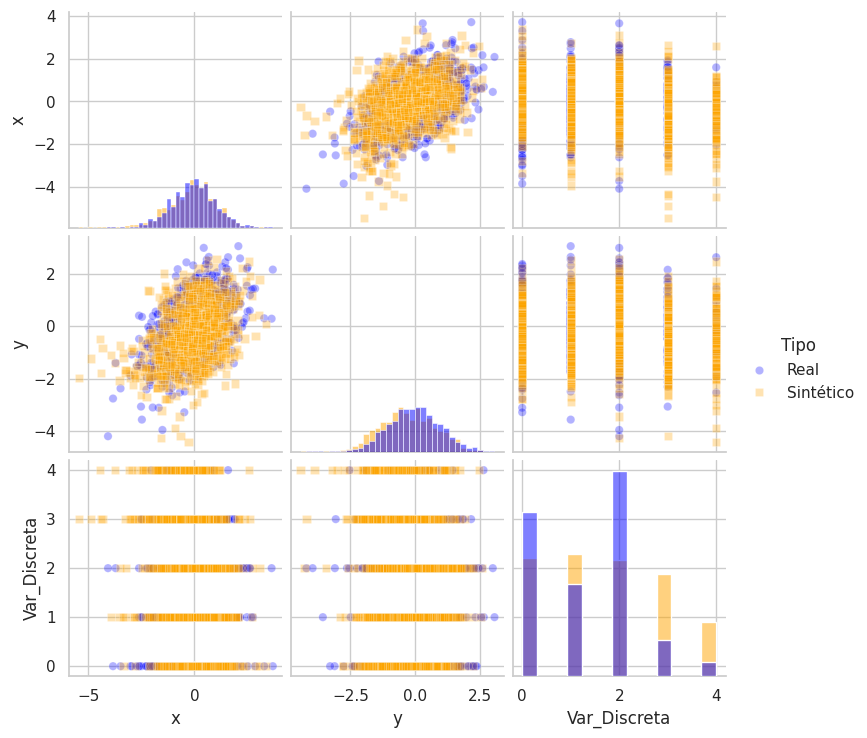
\includegraphics[scale=.35]{figures/4-Advanced_Strategies/pairplot_Dataset1.png}
    \caption{Scatter plot and histogram.}
\end{figure}

\begin{itemize}
    \item KS-Complement x: 0.94
    \item KS-Complement y: 0.887
    \item TV-Complement discrete variable: 0.773
\end{itemize}

For the second test, the Iris dataset has been used, which contains 4 continuous features and 1 categorical feature (encoded as a discrete variable from a finite set). This dataset contains few samples (150 in total), so the estimation of the distribution may be affected by the small amount of real data. It was trained for 1500 epochs in a few seconds. The 'species' variable was encoded as \{ 'setosa': 0, 'versicolor': 1, 'virginica': 2 \}. After training, 150 data points were sampled from the generated distribution:\\

\begin{figure}[htbp]
    \centering
    \begin{minipage}[b]{0.5\textwidth}
      \centering
      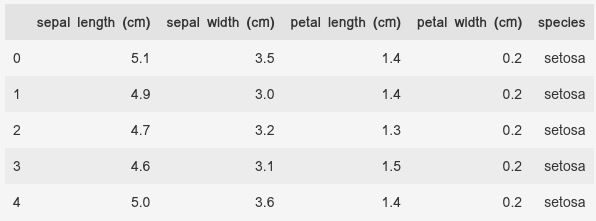
\includegraphics[width=0.7\textwidth]{figures/4-Advanced_Strategies/Ejemplo_Dataset_2_Real.png}
      \caption{Real samples}
    \end{minipage}
    \hfill
    \begin{minipage}[b]{0.5\textwidth}
      \centering
      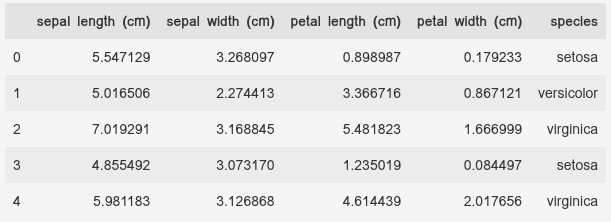
\includegraphics[width=0.7\textwidth]{figures/4-Advanced_Strategies/Ejemplo_Dataset_2_Sintetico.png}
      \caption{Synthetic samples}
    \end{minipage}
\end{figure}

\begin{figure}[H]
    \centering
    \includegraphics*[scale=.3]{figures/4-Advanced_Strategies/pairplot-Dataset2.png}
    \caption{Scatter plot and histogram.}
\end{figure}

\begin{itemize}
    \item KS-Complement sepal length (cm): 0.91
    \item KS-Complement sepal width (cm): 0.85
    \item KS-Complement petal length (cm): 0.89
    \item KS-Complement petal width (cm): 0.8
    \item TV-Complement species: 0.96
\end{itemize}

We observe that in both datasets, a high marginal similarity of the columns has been achieved (close to 1). The scatter plots show that the model has relatively well captured the correlations between variables, and the histograms between real and synthetic data are quite similar. However, good performance in these datasets does not necessarily imply it is a good model. It is currently known that there are models that better capture the distribution of tabular data, although the use of GANs can still be useful in this task. Available resources, such as computing power or the amount of data, will guide the choice between different methods.\\
The generation of synthetic tabular data using GANs can be an additional tool in the set of technologies aiming to train models with sensitive data while safeguarding privacy. The quality of synthetic data depends on many factors: the original dataset size, imbalanced classes, etc. However, these networks seem to approximate the distribution of the original data, though not perfectly. Approximating the joint distribution is a very complex problem to solve, and in this work, only very simple datasets have been used, and even with these datasets, it has not been possible to perfectly approximate the original distribution.\\
This is why, although it is a promising technique, I do not believe it is appropriate to use it for conducting scientific studies or training models solely using synthetic data. Nonetheless, they do fulfill the intended function: serving as a guide for adjusting models in a Federated Learning environment without needing to share the original data. With synthetic data, the different entities that hold the data can share these synthetic data to help researchers understand, albeit approximately, the type of data they need to work with.\\
For this purpose, I believe that data generation can be helpful. It should be studied to what extent generative models can resist attacks aimed at extracting information about the original data (\cite*{sun2023}), although this is beyond the scope of this work.\\

Other techniques for generating synthetic data use architectures different from GANs, such as Variational Autoencoders \cite{xu2019} or simpler statistical models like Gaussian Copulas \cite{li2020a}. For a detailed summary of the various tabular data generation techniques, I recommend checking \cite{papadaki2024}.
